Much of the work done during a page fault, while important, does not strictly
need to occur in order for the application thread to make progress. For
example, allocating free frames or updating page metadata could be performed at
any time. Other tasks may be more efficient in hardware than in the OS; the
walking of page-tables for example. We propose a hardware accelerator that
performs only the bare-minimum of coppying a remote page into a pre-allocated
frame, updating the relevant PTE, and restarting the application (figure
\ref{fig:pfa_generic}).

\begin{figure}[h]
    \centering
    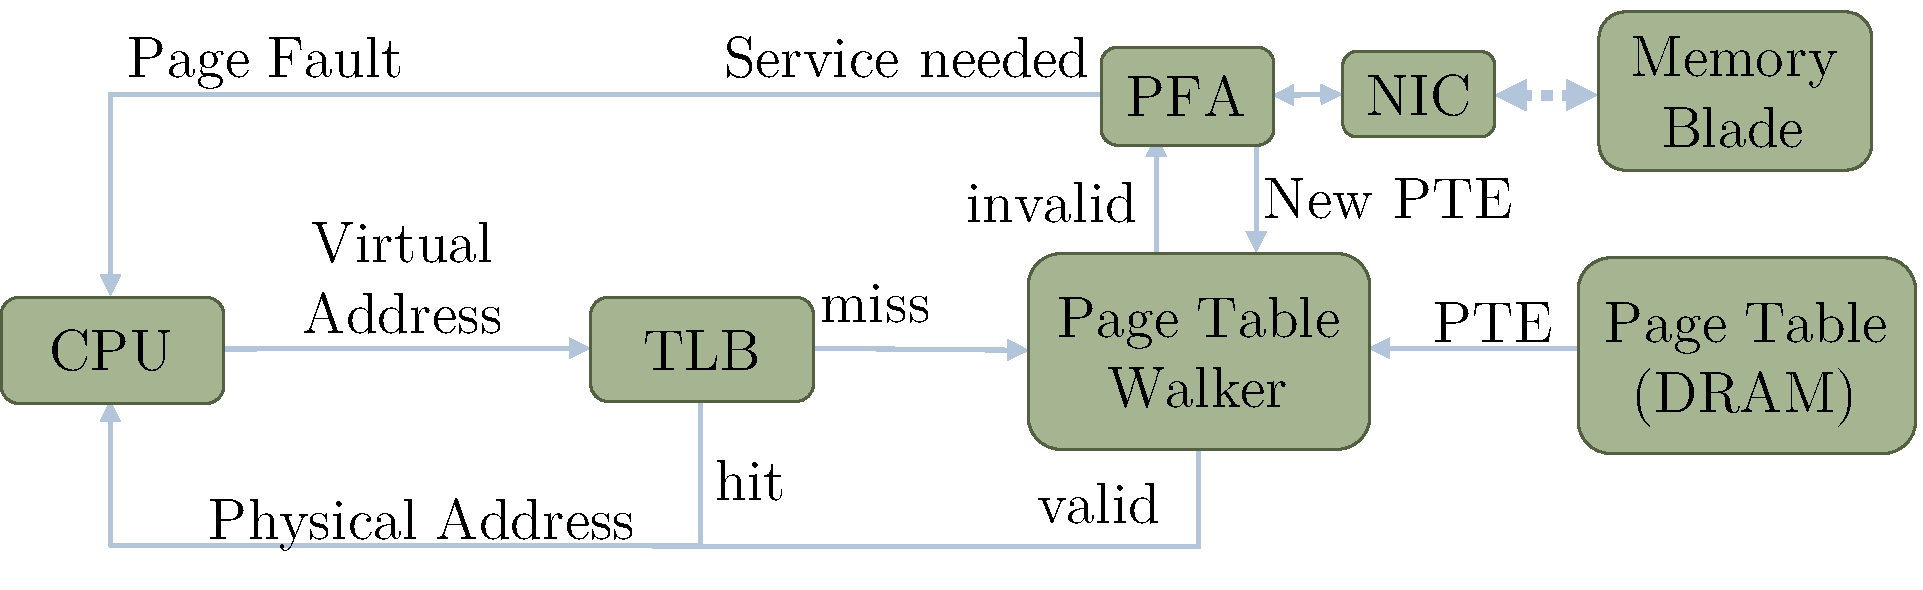
\includegraphics[width=0.9\columnwidth]{figs/generic_pfa.pdf}
    \vspace{-5mm}
    \caption{Paging with the PFA}
    \label{fig:pfa_generic}
\end{figure}

While this does not eliminate the need for software management of page metadata
(here referred to as \gls{bookkeeping}), it does provide considerable flexibility
to the OS in how such \glspl{task} get scheduled. Figure
\ref{fig:bookkeeping_timeline} illustrates the difference from the perspective
of the OS. One immediate benefit is that the OS can schedule this bookkeeping
thread on idle resources, e.g. while the application is blocked on I/O.
Another benefit is that bookkeeping tasks can now be batched. Batching improves
cache locality and amortizes context switch overheads. 

\begin{figure}[h]
    \centering
    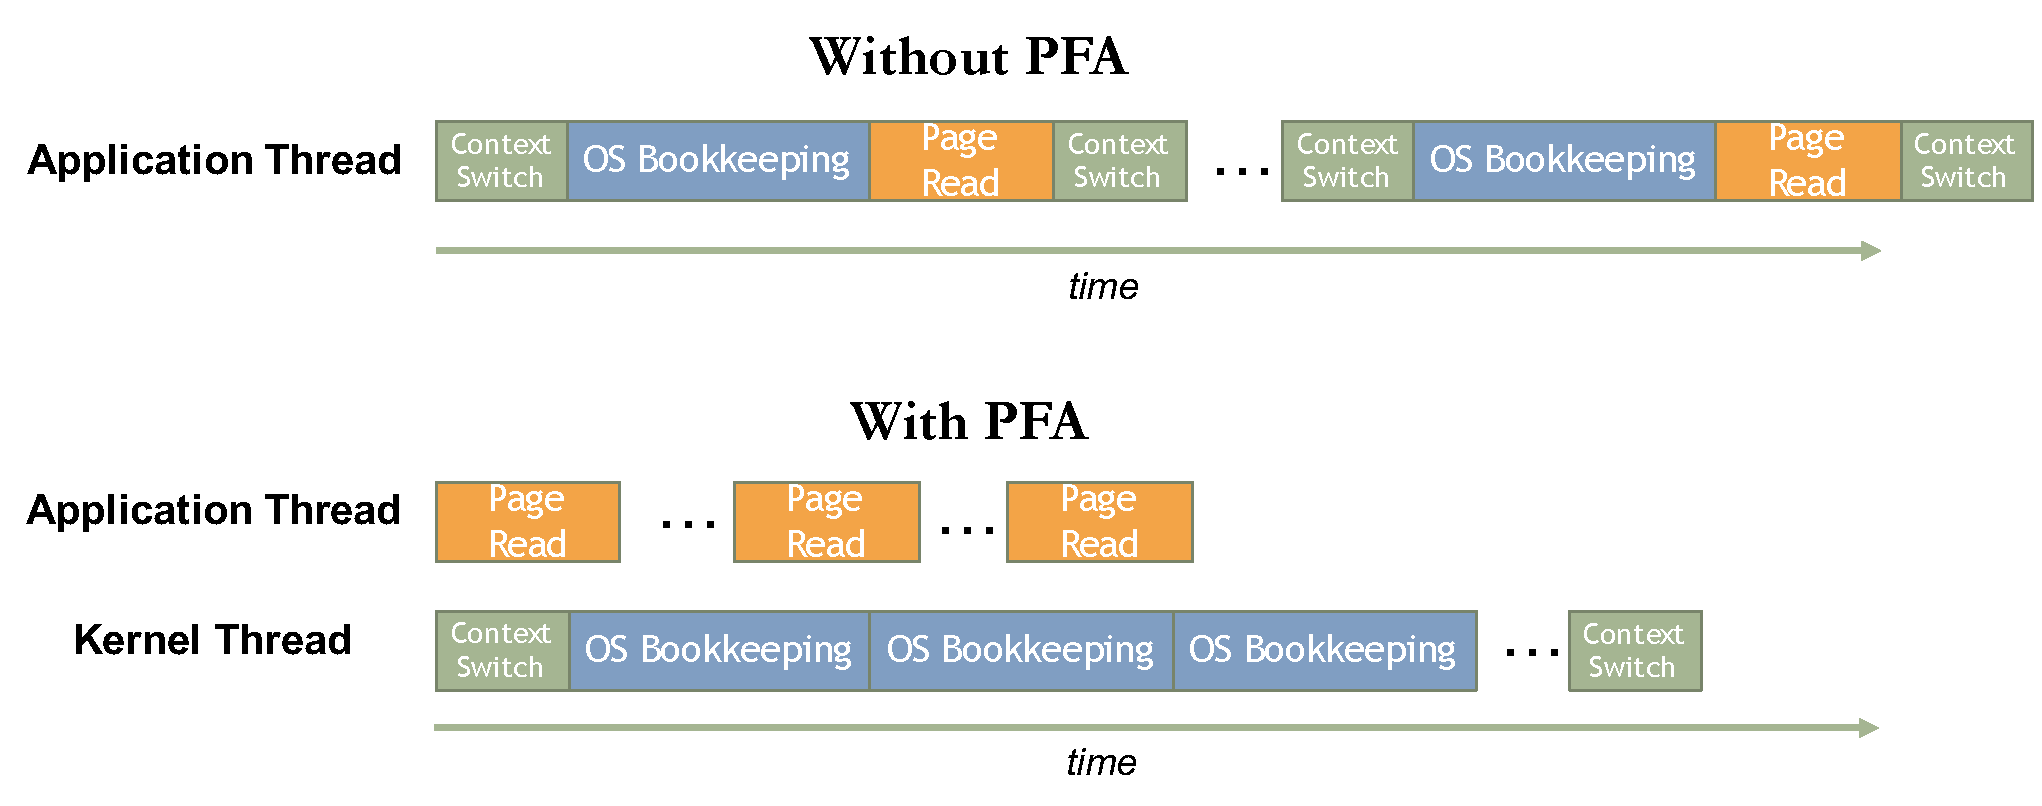
\includegraphics[width=0.9\columnwidth]{figs/bookkeeping_timeline.pdf}
    \vspace{-5mm}
    \caption{Timeline of page-fault processing with and without the PFA}
    \label{fig:bookkeeping_timeline}
\end{figure}

